\chapter{Simulation modes and simulation editors}
\label{sec:simmodes}

OghmaNano uses a modular architecture that enables the core solver to perform a variety of simulation types using \index{plugins}. For example there is a plugin to perform steady state JV simulations, another plugin to perform frequency domain simulations, and another to calculate the Quantum Efficiency. They all leverage the same OghmaNano core solver but run it in a slightly different way with custom inputs and outputs. A list of the plugins and what they do can be found below:

\begin{itemize}
	\vspace{-0.2cm}\item Plugins for various types of experiment
	\begin{itemize}
		\vspace{-0.2cm}\item jv: To calculate steady state JV curves.
		\vspace{-0.2cm}\item suns\_jsc: Simulate suns v.s. Jsc curves.
		\vspace{-0.2cm}\item suns\_voc: Suns v.s. Voc simulations.
		\vspace{-0.2cm}\item eqe: Simulates EQE.
		\vspace{-0.2cm}\item cv: Capacitance voltage simulations.
		\vspace{-0.2cm}\item ce: To simulate charge extraction experiments.
		\vspace{-0.2cm}\item time\_domain: A time domain solver for transient simulations.
		\vspace{-0.2cm}\item fx\_domain: Simulate the frequency domain response of a device, both electrical and optical excitation.
		\vspace{-0.2cm}\item pl\_ss: Calculate the PL spectrum at in steady state.
		\vspace{-0.2cm}\item mode: Used to solve optical modes in 1/2D waveguides.
		\vspace{-0.2cm}\item spm: Simulates scanning probe microscopy in 3D electrical simulations.
		\vspace{-0.2cm}\item equilibrium: Equilibrium electrical simulations.
		\vspace{-0.2cm}\item exciton: Exciton simulations.
		\vspace{-0.2cm}\item mesh\_gen: Generates meshes.
	\end{itemize}
	\vspace{-0.2cm}\item Optical solver plugins
	\begin{itemize}
		\vspace{-0.2cm}\item fdtd: Finite Difference Time Domain (FDTD) optical solver.
		\vspace{-0.2cm}\item optics: Optical transfer matrix solver for 1D structures
		\vspace{-0.2cm}\item light\_full: Optical transfer matrix solver.
		\vspace{-0.2cm}\item light\_qe: Calculates optical profile using the experimental quantum efficiency.
		\vspace{-0.2cm}\item light\_exp: Calculates optical profile assuming exponential propagation of light in 1D structures.
		\vspace{-0.2cm}\item light\_flat: Calculates optical profile assuming flat optical profiles in the structure.
		\vspace{-0.2cm}\item light\_constant: Assumes user given values of generation rate in optical structures.
		\vspace{-0.2cm}\item light\_fromfile: Takes a generation rate from a file.
	\end{itemize}
\end{itemize}

In the simulation editors ribbon (see Figure \ref{fig:simeditors}) you can see icons that represent each plugin, these are the simulation editors. By clicking on an icon in this ribbon you will be able to edit how the plugin performs the various simulations.  For example in the JV simulation editor one can change the start/stop voltages of a voltage sweep.  The JV editor can be seen in Figure \ref{fig:jv_low}. Within each simulation editor the user can define multiple so called \emph{experiments}. This can be seen in below in Figure \ref{fig:jv_low} and Figure \ref{fig:jv_high}, where two JV scans have been defined within the JV editor, one called \emph{JV curve - low voltage} and another called \emph{JV curve - high voltage}. One has a start voltage of 0.02V and stop voltage of 1.0V, while the other has a start voltage of 1.0V and a stop voltage of 10V.  This feature is most useful in more complex experiments such as in time domain experiments where one may want to simulate multiple different voltage/light ramps/pulses for one device. There is no limit to how many \emph{experiments} can be defined for each plugin.
\\
\begin{figure}
\centering
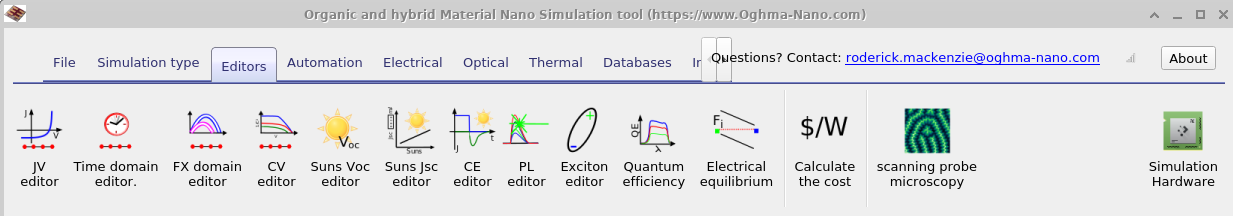
\includegraphics[width=\linewidth,height=0.2\linewidth]{./images/sim_editors/ribbon_sim_editors.png}
\caption{Simulation editors use this toolbar to edit the various simulation conditions your device will experience.}
\label{fig:simeditors}
\end{figure}

\begin{minipage}{0.5\textwidth}
	\centering
	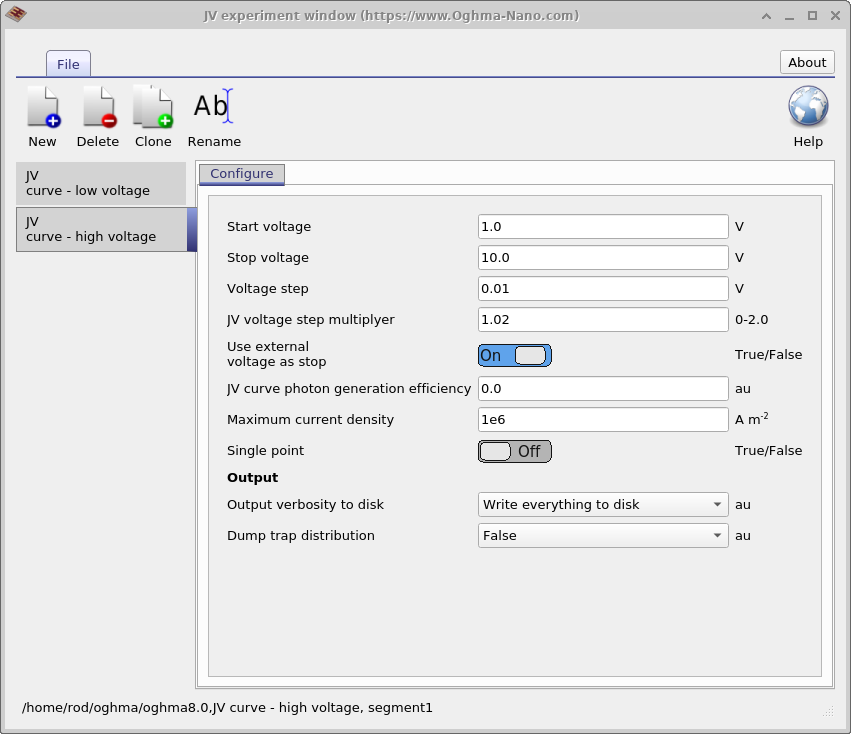
\includegraphics[width=\linewidth,height=0.8\linewidth]{./images/sim_editors/jv_high_voltage.png}
	\captionof{figure}{An experiment set up in the JV window for high voltage simulations.}
	\label{fig:jv_low}
\end{minipage}
\hspace{4pt}
\begin{minipage}[]{0.5\linewidth}
	\centering
	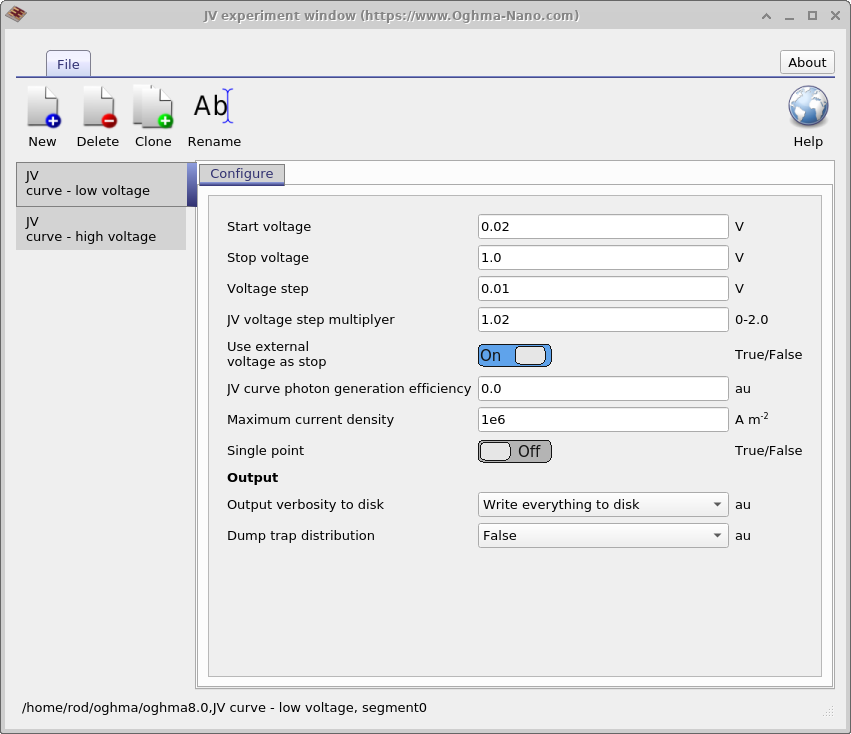
\includegraphics[width=\linewidth,height=0.8\linewidth]{./images/sim_editors/jv_low_voltage.png}
	\captionof{figure}{An experiment set up in the JV window for low voltage simulations.}
	\label{fig:jv_high}
\end{minipage}

Once an \emph{experiment} has been defined an icon representing it will appear in the simulation mode ribbon shown in figure \ref{fig:simmodes}. You can see in the figure an icon for \emph{JV curve low voltage} and \emph{JV curve high voltage} that were defined in Figure \ref{fig:jv_low} and \ref{fig:jv_high}. You can see in Figure \ref{fig:simmodes} that \emph{JV curve low voltage} is depressed. This means that when the simulation is run this simulation mode will be executed. If you select another simulation mode, then when the play button (or F9) is pressed that simulation mode will be run. Only one simulation mode can be run at a time.


\begin{figure}[H]
\centering
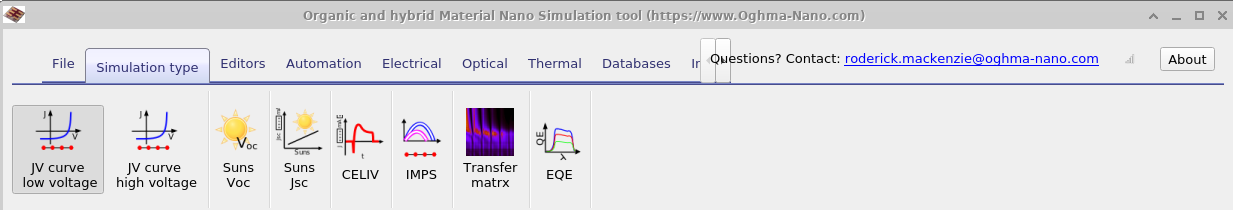
\includegraphics[width=\linewidth,height=0.2\linewidth]{./images/sim_editors/ribbon_sim_modes.png}
\caption{Selecting a simulation mode, in this case the \emph{JV curve low voltage} has been selected so that when the user presses play that simulation mode will be run.}
\label{fig:simmodes}
\end{figure}

\newpage
\section{JV editor (Steady state simulation editor)}
If you click on the JV editor icon in figure \ref{fig:ribbon_jv}, the JV editor window will open shown below in figure \ref{fig:jvcurveeditor}.

\begin{figure}[H]
\centering
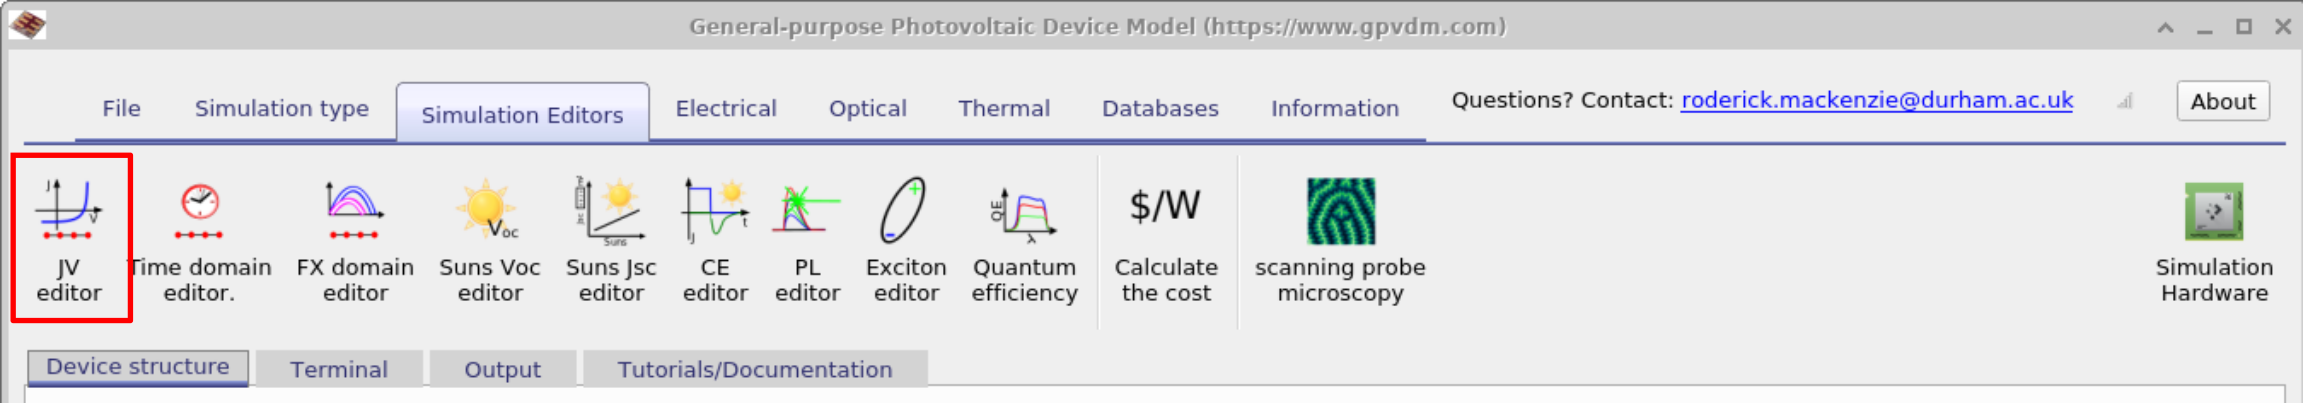
\includegraphics[width=0.8\textwidth]{./images/sim_editors/ribbon_jv.png}
\caption{Opening the JV editor from the simulation editor ribbon.}
\label{fig:ribbon_jv}
\end{figure}

This window can be used to configure steady state simulations. It does not matter if you are running a current-voltage sweep on a solar cell or an OFET.  This plugin will steadily ramp the voltage from a start voltage to a stop voltage.  The voltage will be applied to the \emph{active} contact as defined in the \emph{contact editor}.  You can set the start voltage, stop voltage and step size.  Use \emph{JV voltage step multiplayer} to make the voltage step grow each step.  The default is 1.0, i.e. no growth.

\begin{figure}[H]
\centering
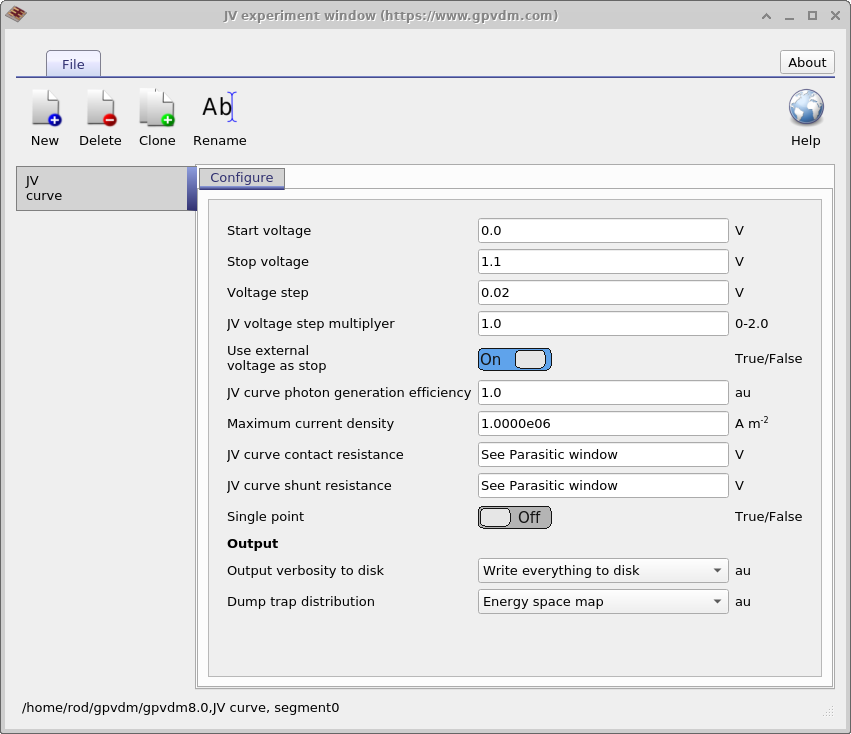
\includegraphics[width=0.7\textwidth,height=0.6\textwidth]{./images/sim_editors/jv_editor.png}
\caption{The JV editor editor window, use this to configure steady state simulations.}
\label{fig:jvcurveeditor}
\end{figure}

The files produced by the JV simulation mode are given in table \ref{tab:jv_output}.

\begin{table}[H]
\begin{center}
\begin{tabular}{ |c|c|c| } 
 \hline
	File name 			& 	Description  \\ 
 \hline
	$jv.dat$ 			&	Current voltage curve \\ 
	$charge.dat$ 		&	voltage charge density\\ 
	$k.csv$ 			&	Recombination constant k\\ 
	$sim\_info.dat$ 	&	Calculated $V_{oc}$, $J_{sc}$ etc.. see \ref{sec:siminfo}   \\

 \hline
\end{tabular}
\caption{Files produced by the JV simulation}
\label{tab:jv_output}
\end{center}
\end{table}



\newpage
\section{Time domain editor}
Related YouTube videos:
\begin{figure}[H]

\begin{tabular}{ c l }


\includegraphics[width=0.05\textwidth]{./images/youtube.png}

&
\href{https://www.youtube.com/watch?v=D7yJLFmTAVQ}{Simulating optoelectronic sensors made from polymers.}

\end{tabular}
\end{figure}

The time domain editor can be used to configure time domain simulations, this is shown in figure \ref{fig:timedomaineditor}.  You can see that one simulation editor can be used to edit multiple simulations.  The panel on the left shows the editor being used to edit a CELIV simulation while the panel on the right shows the editor being used to edit a TPC simulation.  The new, delete and clone buttons in the top of the window can be used to make new simulation modes. The table in the bottom of the window can be used to setup the time domain mesh, apply voltages or light pulses.

\begin{figure}[H]
\centering
\begin{tabular}{ c c }

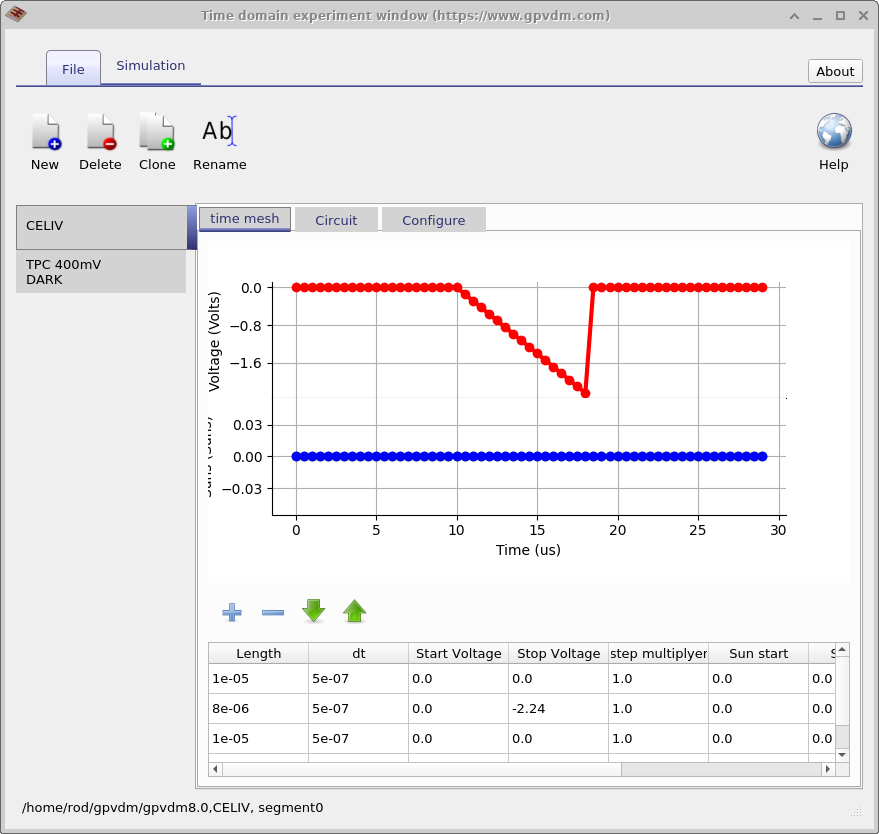
\includegraphics[width=0.5\textwidth,height=0.4\textwidth]{./images/time_domain_editor.png}

&
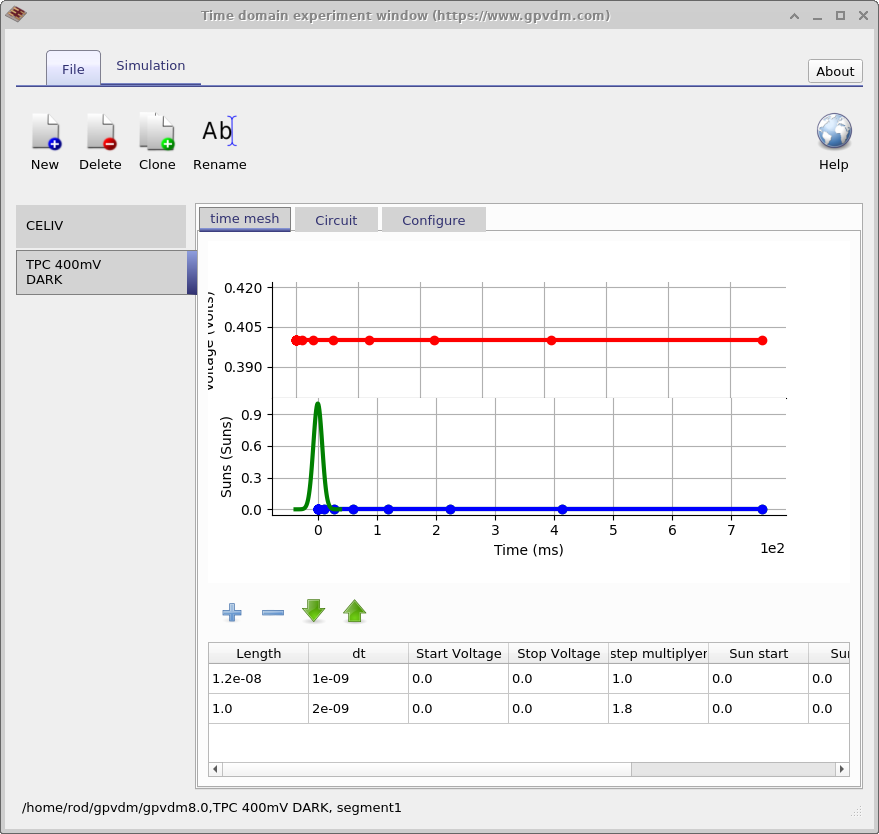
\includegraphics[width=0.5\textwidth,height=0.4\textwidth]{./images/time_domain_editor2.png}

\\

\end{tabular}
\caption{The time domain editor showing the user editing the duration of light/voltage pulses.}
\label{fig:timedomaineditor}
\end{figure}

Figure \ref{fig:timedomaineditor2} shows different tabs in of the time domain editor. The image on the left shows the circuit diagram used to model the CELIV experiment. From the left of the image the diode on the left accounts for the drift diffusion simulations it is in effect a perfect diode.  Then comes a capacitor used to model the charge on the plates of the device, then a shunt resistance and then the series resistance.  The final resistor on the right represents the external resistance of the measuring equipment.  The right hand figure shows the configuration options of the time domain window.

\begin{figure}[H]
\centering
\begin{tabular}{ c c }

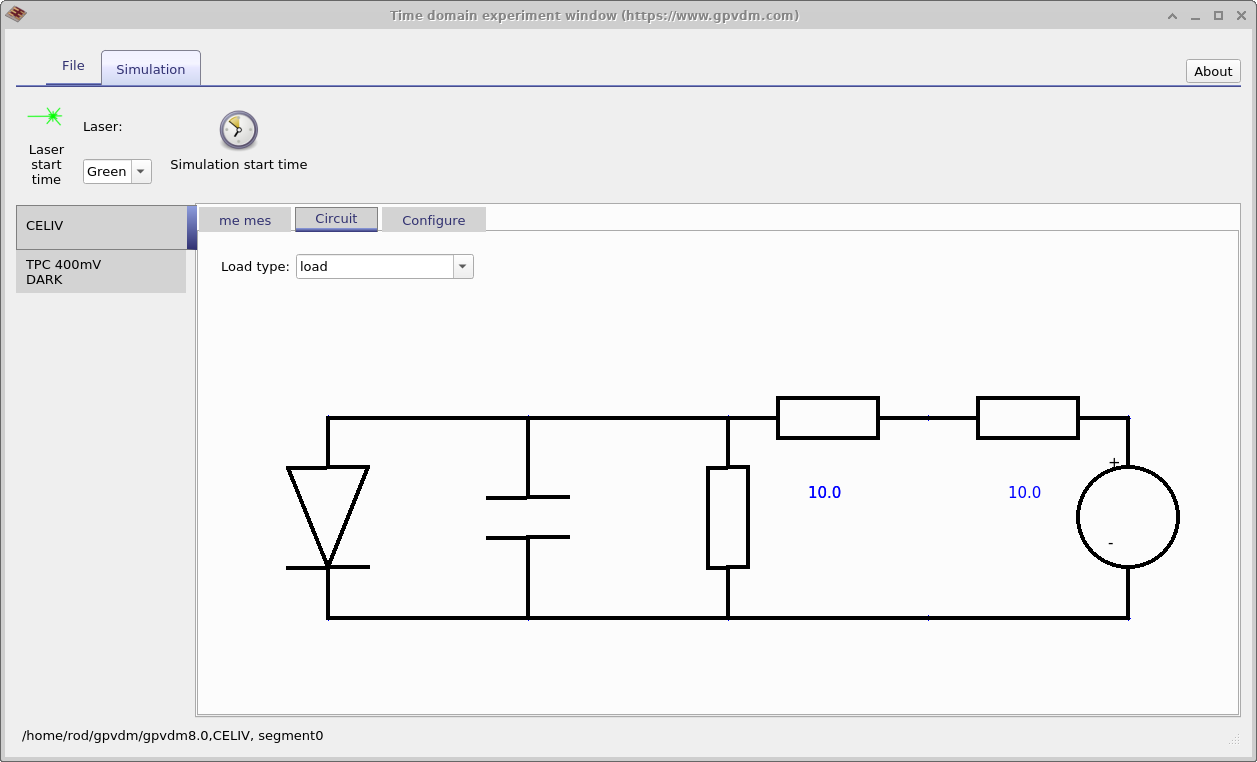
\includegraphics[width=0.5\textwidth,height=0.4\textwidth]{./images/time_domain_editor1.png}

&
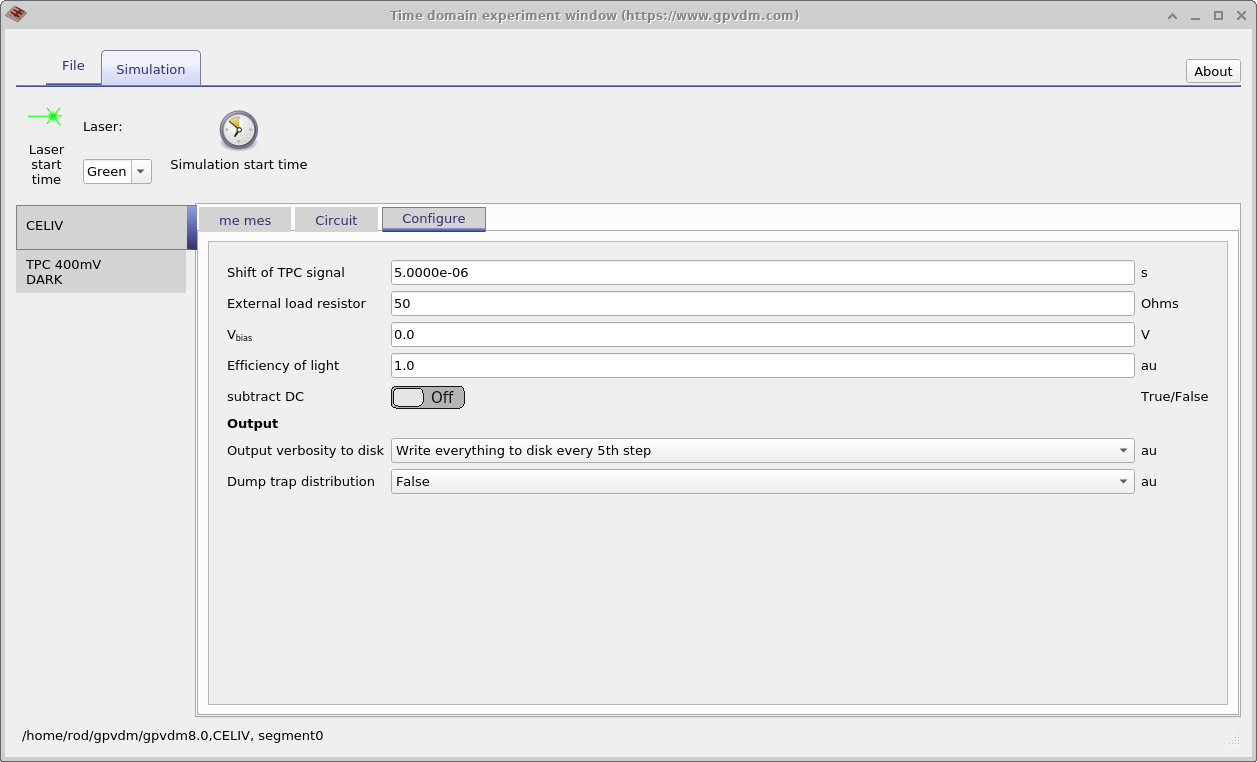
\includegraphics[width=0.5\textwidth,height=0.4\textwidth]{./images/time_domain_editor4.png}

\\

\end{tabular}
\caption{Configuring the time domain editor}
\label{fig:timedomaineditor2}
\end{figure}

\newpage
\section{Frequency domain editor}
Related YouTube videos:
\begin{figure}[H]

\begin{tabular}{ c l }


\includegraphics[width=0.05\textwidth]{./images/youtube.png}

&
\href{https://www.youtube.com/watch?v=NJAsZeiB5FU}{Simulating impedance spectroscopy (IS) in solar cells.}

\end{tabular}
\end{figure}

\subsection{Overview}
The frequency plugin allows you to simulate the frequency domain response of the device.  Using this tool one can perform impedance spectroscopy, as well as optically excited measurements such as Intensity Modulated Photo Spectroscopy (IMPS), Intensity Modulated Voltage Spectroscopy (IMVS). The  domain editor allows you to configure frequency domain simulations. This is shown below in Figures \ref{fig:fx_domain_mesh} and \ref{fig:fx_domain_circuit}. On the left hand side is the frequency domain mesh editor this is used to define which frequencies will be simulated.  Figure \ref{fig:fx_domain_circuit} shows the \emph{circuit} tab of the frequency domain window, this sets the electrical configuration of the simulation. One can either simulate an ideal diode (this is the fastest type of simulation to perform), a diode with parasitic components or a diode in open circuit. An ideal diode would be used for IMPS simulations while the open circuit model would be used for IMVS simulations. Pick the circuit depending on what conditions you want to simulate. If you want examples of frequency domain simulation look in the new simulation window under Organic Solar cells, some of the PM6:Y6 devices have examples of frequency domain simulations already set up.
\\
\\
\noindent
\begin{minipage}{0.5\textwidth}
	\centering
	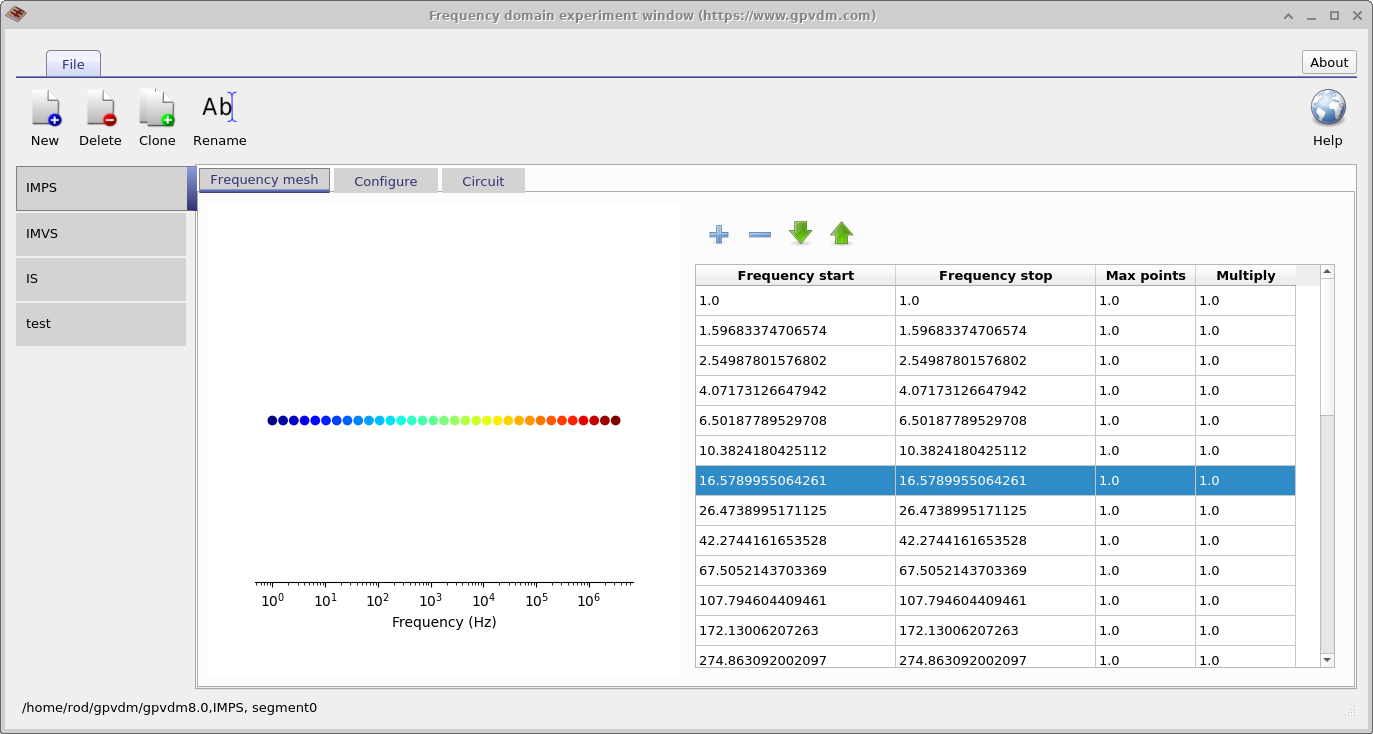
\includegraphics[width=\linewidth,height=0.8\linewidth]{./images/sim_editors/fx_domain_editor.png}
	\captionof{figure}{The frequency domain editor window}
	\label{fig:fx_domain_mesh}
\end{minipage}
\hspace{4pt}
\begin{minipage}[]{0.5\linewidth}
	\centering
	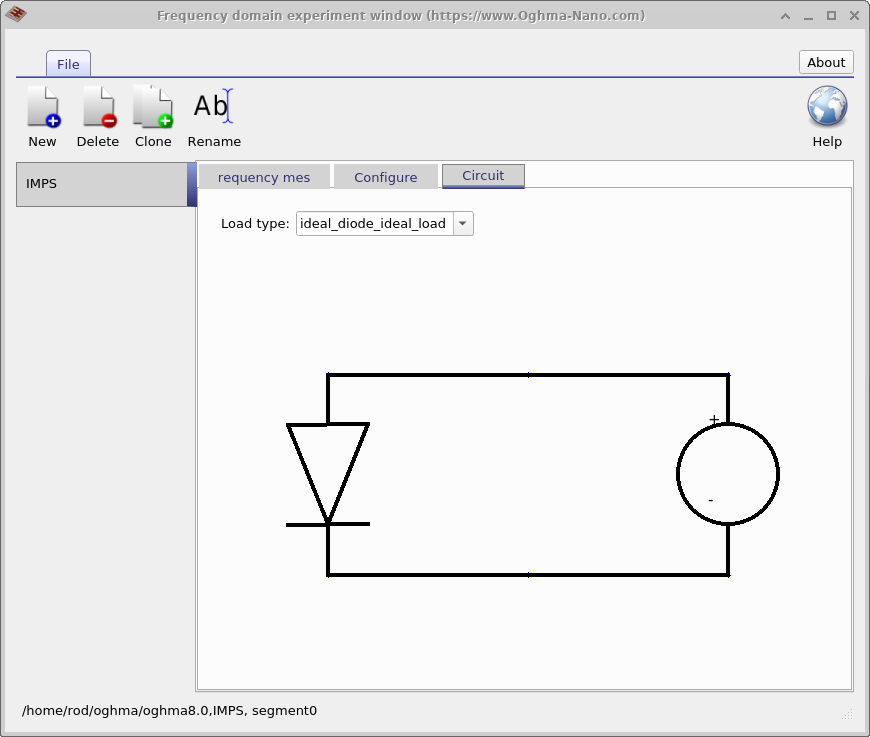
\includegraphics[width=\linewidth,height=0.8\linewidth]{./images/sim_editors/fx_domain_circuit.png}
	\captionof{figure}{A circuit set up for frequency domain simulations.}
	\label{fig:fx_domain_circuit}
\end{minipage}

\subsubsection{Large signal or small signal}
There are two ways to simulate frequency domain simulations in a device model, a large signal approach or a small signal approach. The small signal approach assumes the problem we are looking at varies linearly around a DC point, this may or may not be true depending on the conditions one is looking at. This method is however computationally fast.  The second approach is to use a large signal approach and rather than simulating linear variation around a set point one simulates the time domain response of the device in full for each wavelength of interest.  This method is cope better non-linear systems and one does not need to worry if one is in the large or small signal regime but is slower.  OghmaNano uses the large signal approach.

\subsection{Inputs}
In Figure \ref{fig:fx_domain_option} the \emph{Configure} tab of the frequency domain window can be seen. This decides exactly how the simulation will perform. These are described below in table \ref{tab:fx_inputs}

\begin{table}
\begin{center}
\begin{tabular}{ |l|p{8cm}| } 
 \hline
	File name 					& 	Description  \\ 
 \hline
	$V_{external}$				&	The external voltage applied to the cell\\ 
	Simulation type				&	Leave this as Large signal.\\
	Load resistor				&	External load resistor, this should be usually set to zero.\\ 
	FX domain mesh points 		&	The number of time steps used to simulate each cycle\\ 
	Cycles to simulate 			&	The number of complete periods of any given frequency that are simulated \\ 
	Excite with					&	How the device is excited, either optically or electrically.\\ 
	Measure 					&	What is measured, current or voltage.\\
	Modulation depth			&	How deep is the DC voltage/current modulated\\
 	Periods to fit				&	The number of frequency domain cycles that are fit to extract phase angle\\
 	Output verbosity to disk	&	How much data is dumped to disk (described in other sections)\\
 	Output verbosity to screen	&	How much data is shown on the creen (described in other sections)\\
 \hline
\end{tabular}
\caption{Files produced by the time domain simulation}
\label{tab:fx_inputs}
\end{center}
\end{table}

\begin{figure}
\centering
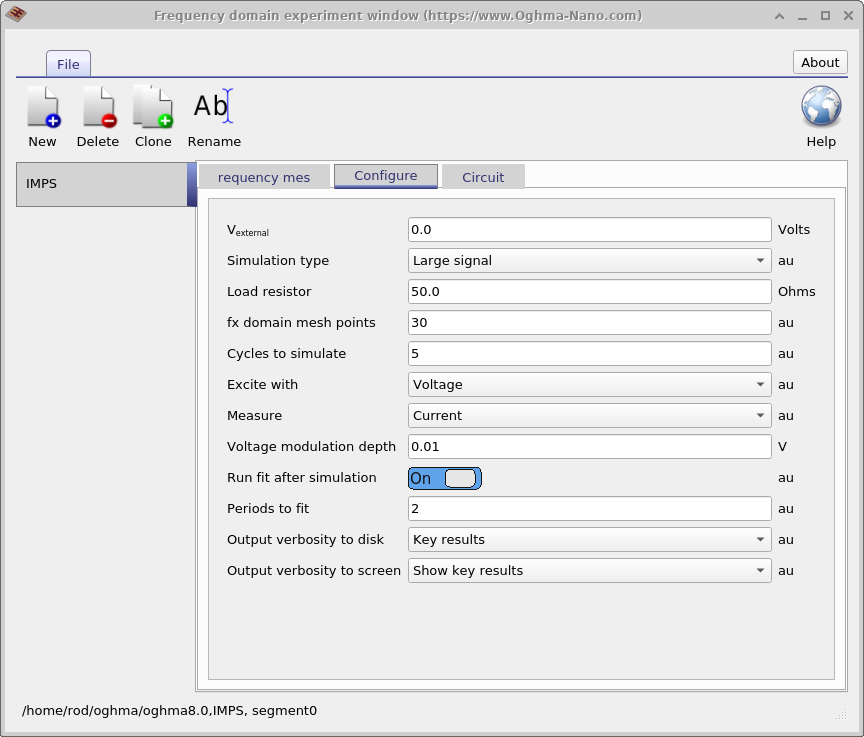
\includegraphics[width=0.7\linewidth,height=0.5\linewidth]{./images/sim_editors/fx_domain_options.png}
\caption{Configuring a frequency domain simulation}
\label{fig:fx_domain_option}
\end{figure}


\subsection{Outputs}


\begin{table}[H]
\begin{center}
\begin{tabular}{ |c|c|c| } 
 \hline
	File name 			& 	Description  \\ 
 \hline
	real\_imag.csv		&	Re(i(fx)) v.s. Im(i(fx))\\ 
	fx\_imag.csv		&	fx v.s. Im(i(fx))\\
	fx\_real.csv 		&	fx v.s. Re(i(fx))\\ 
	fx\_abs.csv 		&	fx v.s. $\lvert i(fx) \rvert$\\ 
	fx\_phi.csv 		&	fx v.s. $ \angle i(fx)$ \\ 
	fx\_C.csv 			&	fx v.s. Capacitance\\ 
	fx\_R.csv 			&	fx v.s. Resistance\\ 
 \hline
\end{tabular}
\caption{Files produced by the time domain simulation}
\label{tab:ce_output}
\end{center}
\end{table}


\clearpage
\section{Suns-Voc editor}
The Suns-Voc plugin can be used to calculate how open circuit voltage changes as a function of light intensity.  This can be useful for understanding tail slope and disorder in devices.  A picture of the suns-voc editor window can be seen below in figure \ref{fig:sunsvoceditor}.  The window can be used to set the start and stop light intensity. The Suns-Voc applies the voltage to the contact that is labelled \emph{Change}.

\begin{figure}[H]
\centering
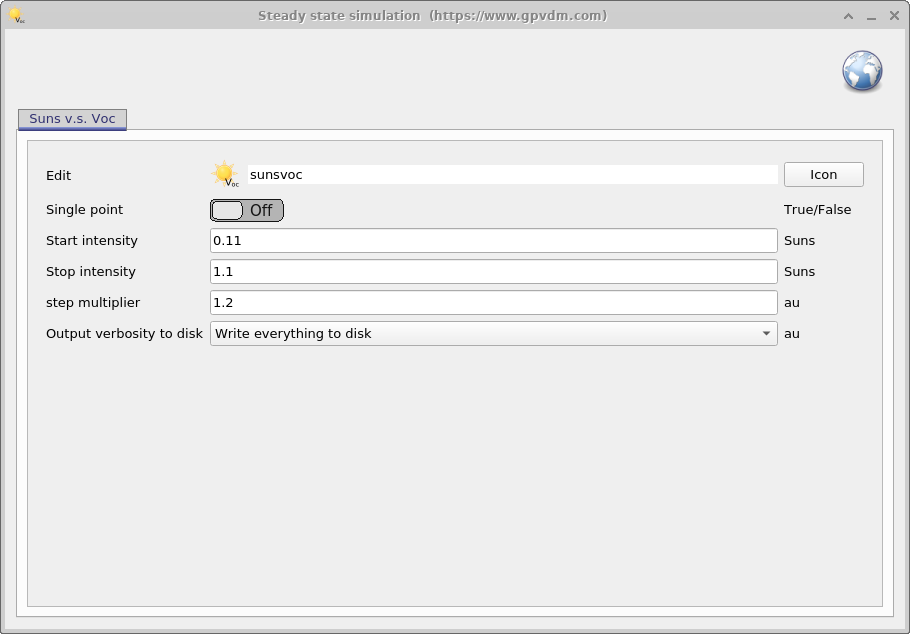
\includegraphics[width=0.7\textwidth,height=0.5\textwidth]{./images/sim_editors/suns_voc_editor.png}
\caption{The suns-voc editor window}
\label{fig:sunsvoceditor}
\end{figure}


\subsection{Outputs}

\begin{table}[H]
\begin{center}
\begin{tabular}{ |c|c| } 
 \hline
	File name 			& 	Description  \\ 
 \hline
	suns\_voc.csv 		&	Suns v.s. Voc curve \\ 
	suns\_Q.csv 		&	Suns v.s. Charge density\\ 
	suns\_mu.csv 		&	Suns v.s. average charge carrier mobility\\
	suns\_tau.csv 		&	Suns v.s. recombination constant tau \\ 
	Q\_Qtau.csv 		&	Charge density v.s. recombination constant tau \\
	Q\_mu.csv 			&	Charge density v.s. charge carrier mobility\\
	Q\_kbi.csv 			&	Charge density v.s. recombination prefactor kbi\\
	Q\_trap\_filling.csv &	Charge density v.s. fraction of filled traps\\
	V\_mu.csv 			&	Voc v.s. average charge carrier mobility\\
 \hline
\end{tabular}
\caption{Files produced by the Suns-Voc simulation}
\label{tab:suns_voc_output}
\end{center}
\end{table}


\newpage
\section{Suns-Jsc editor}
The Jsc editor can be used to configure suns-Jsc simulations. It enables you to set the start light intensity, stop light intensity and how big the steps are. This is shown in figure \ref{fig:sunsjsceditor}.

\begin{figure}[H]
\centering
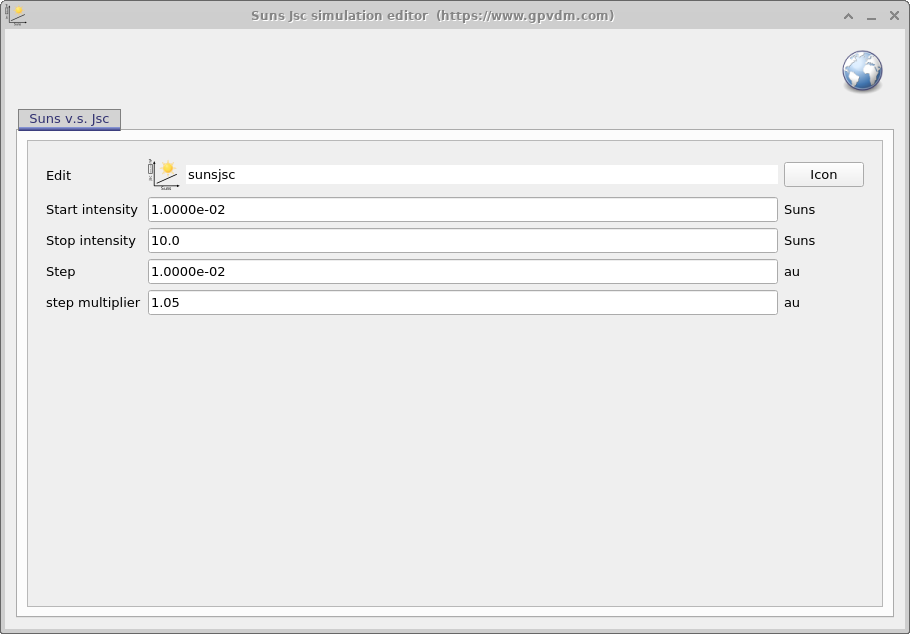
\includegraphics[width=0.7\textwidth,height=0.5\textwidth]{./images/sim_editors/suns_jsc_editor.png}
\caption{The JV curve editor window}
\label{fig:sunsjsceditor}
\end{figure}


\subsection{Outputs}

\begin{table}[H]
\begin{center}
\begin{tabular}{ |c|c| } 
 \hline
	File name 		& 	Description  \\ 
 \hline
	suns\_jsc.csv 	&	Suns v.s. Jsc curve \\ 
	suns\_mu.csv		&	Suns v.s. average charge carrier mobility \\ 
 \hline
\end{tabular}
\caption{Files produced by the Suns-Jsc simulation}
\label{tab:suns_jsc_output}
\end{center}
\end{table}

\clearpage
\section{Quantum efficiency editor}
The quantum efficiency editor simulates both EQE and IQE.  The configuration window can be used to set the voltage at which EQE and IQE are performed.
\begin{figure}[H]
\centering
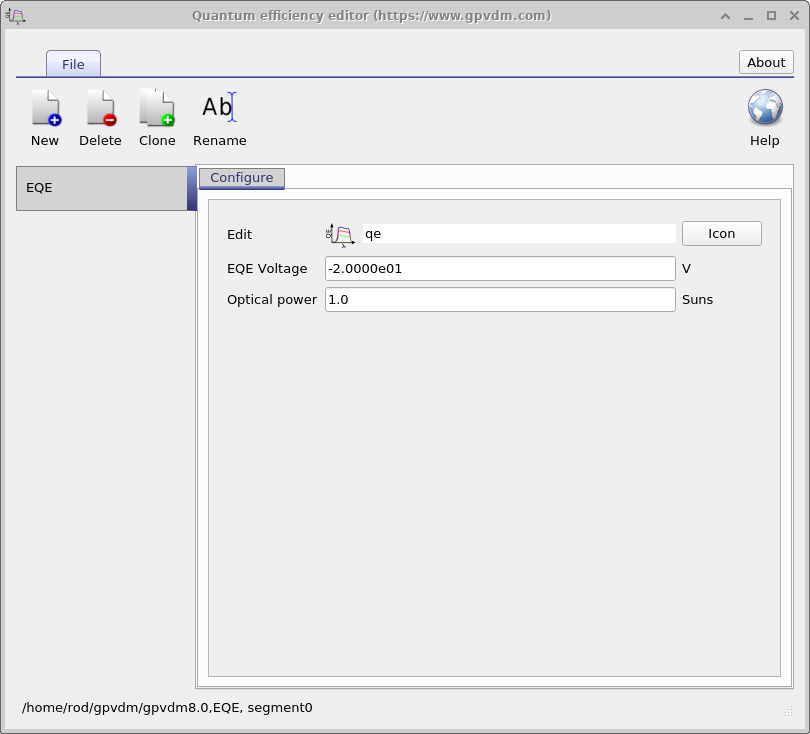
\includegraphics[width=0.7\textwidth,height=0.5\textwidth]{./images/sim_editors/qe_editor.png}
\caption{The quantum efficiency editor window}
\label{fig:qeeditor}
\end{figure}

\subsection{Outputs}

\begin{table}[H]
\begin{center}
\begin{tabular}{ |c|c| } 
 \hline
	File name 		& 	Description  \\ 
 \hline
	eqe.csv 		&	Wavelength v.s. EQE \\ 
	E\_eqe.csv		&	Photon energy v.s. EQE \\ 
	E\_eqe\_norm.csv	&	Photon energy v.s. Normalized EQE  \\ 
	iqe.csv			&	Wavelength v.s. IQE \\ 
	E\_iqe.csv		&	Photon energy v.s. IQE \\ 
	lam\_Gn.csv		&	Wavelength v.s. Average charge carrier generation rate \\ 
 \hline
\end{tabular}
\caption{Files produced by the Suns-Jsc simulation}
\label{tab:suns_jsc_output}
\end{center}
\end{table}

\newpage
\section{Scanning probe microscopy editor}
When simulating a 3D structure such as a large area contact one often wants to map the resistance between an x,z point on the surface of the device and the charge extraction contact. This tool is used to apply voltages systematically over z,x regions to map out voltage or resistance profiles in space.  This tool is usually used with either full 2/3D drift diffusion simulations or the 3D large area electrical circuit model. There is more about this tool in Section \ref{ref:la}.

\begin{figure}[H]
\centering
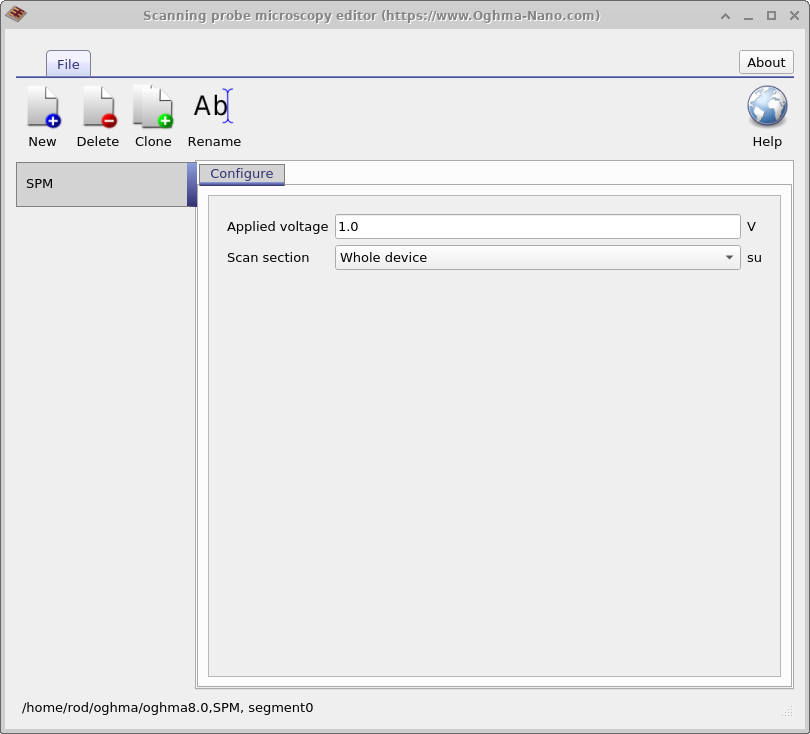
\includegraphics[width=0.7\textwidth,height=0.5\textwidth]{./images/sim_editors/spm.png}
\caption{The scanning probe microscopy editor}
\label{fig:spm_editor}
\end{figure}

\newpage
\section{Electrical equilibrium editor}
Sometimes when studding a device, it is not necessary to simulate an entire JV curve. One may for example just for example be interested in the band structure at 0V in the dark. The \emph{Electrical equilibrium} allows the user to setup simulations that only simulate the device at equilibrium (0V applied bias in the dark).

\begin{figure}[H]
\centering
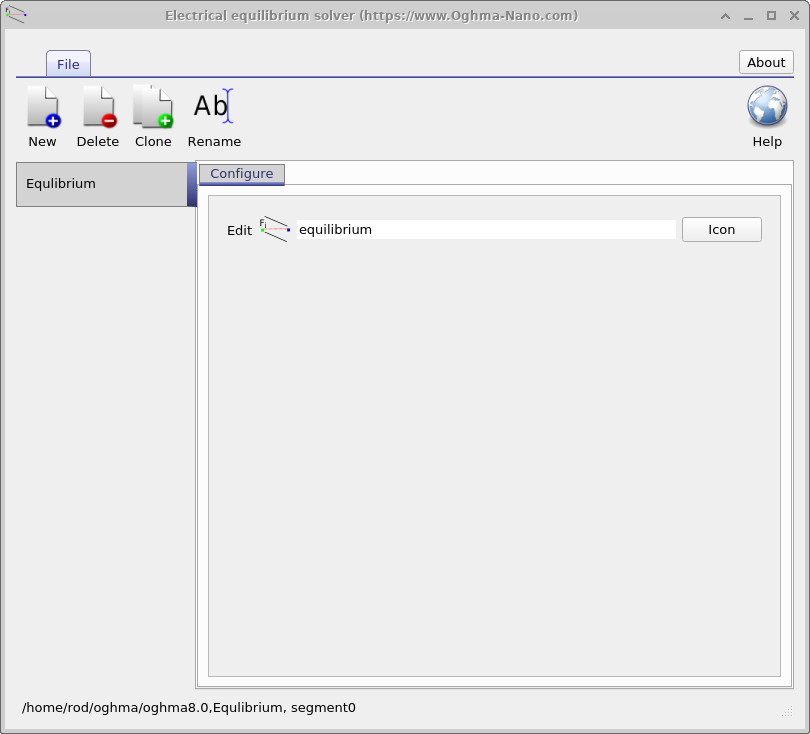
\includegraphics[width=0.7\textwidth,height=0.5\textwidth]{./images/sim_editors/equilibrium.png}
\caption{Electrical equilibrium editor}
\label{fig:equilibrium_editor}
\end{figure}

\newpage
\section{Steady state photoluminencense editor}
This tool is used to generate photoluminencense spectra at a desired voltage, either short circuit or open circuit.

\begin{figure}[H]
\centering
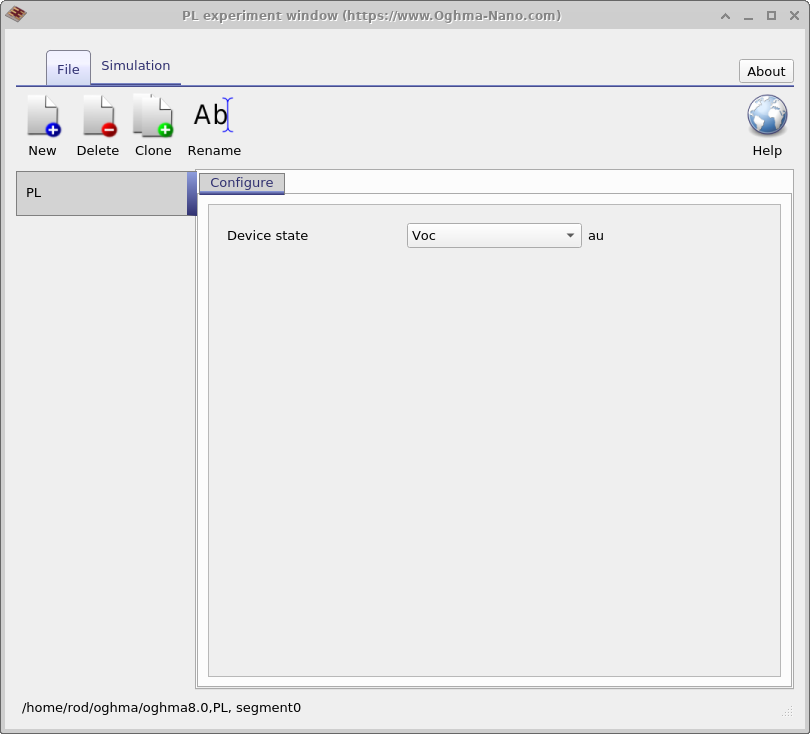
\includegraphics[width=0.7\textwidth,height=0.5\textwidth]{./images/sim_editors/pl.png}
\caption{Steady state photoluminencense editor}
\label{fig:pleditor}
\end{figure}

\newpage
\section{Charge extraction editor}
\noindent
\begin{minipage}{0.5\textwidth}
This is the charge extraction editor, it allows one to simulate charge extraction transients. A charge extraction experiment is performed to find out how much charge is in a disordered device. For this type of experiment one runs the device at a set voltage and light intensity say 1V @ 1Sun. Then one turns off the light and shorts the cell through a resistor and integrates the total current outputted by the cell to get the charge that was in the cell when it was operating. Typically the cell is shorted through the the 50 Ohm termination of an oscilloscope so that by measuring the voltage transient and applying V=IR one can calculate the current and thus total charge.
\end{minipage}
\hspace{4pt}
\begin{minipage}[]{0.5\linewidth}
	\centering
	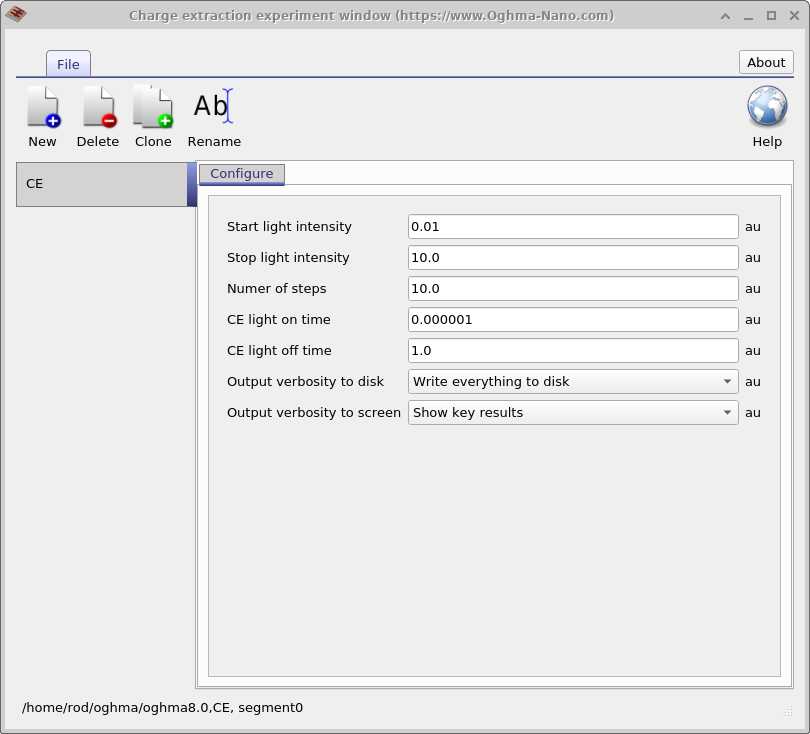
\includegraphics[width=\linewidth,height=0.8\linewidth]{./images/sim_editors/ce.png}
	\captionof{figure}{Charge extraction editor}
	\label{fig:ce_editor}
\end{minipage}
\\
\\
 This type of measurement is important in disordered devices when one wants to find out how much charge is in the trap states.  It is important to note that the experiment does not extract all the charge in the device, it only extracts the difference between charge at operating conditions and 0V @ 0 Suns. The background charge due to injection from the contacts/doping is still left in the device. There is also error loss in the CE experiment due to recombination annihilating charge before it has left the device.


\subsection{Outputs}


\begin{table}[H]
\begin{center}
\begin{tabular}{ |c|c|c| } 
 \hline
	File name 			& 	Description  \\ 
 \hline
	$time\_i.csv$ 		&	Time v.s. extraction current for a single CE experiment\\ 
	$time\_v.csv$ 		&	Time v.s. voltage for a single CE experiment\\ 
	$suns\_Q\_ce.dat$ 	&	Suns v.s. extracted charge including effects of recombination\\ 
	$v\_np.dat$ 			&	Voltage c.s. extracted charge including the effects of recombination \\
	$suns\_np.dat$ 		&	Suns c.s. extracted charge including the effects of recombination   \\
	$v\_np\_ideal.dat$ 	&	Voltage v.s. extracted charge not including the effects of recombination\\
	$suns\_np\_ideal.dat$ &	Suns v.s. extracted charge not including the effects of recombination\\
 \hline
\end{tabular}
\caption{Files produced by the charge extraction simulation}
\label{tab:ce_output}
\end{center}
\end{table}

\clearpage
\section{Capacitance voltage editor}
Experimentally capacitance voltage (CV) measurements are a useful way to determine doping within a device. In OghmaNano CV measurements use a cut down version of frequency domain simulation tool described above.

\begin{figure}[H]
\centering
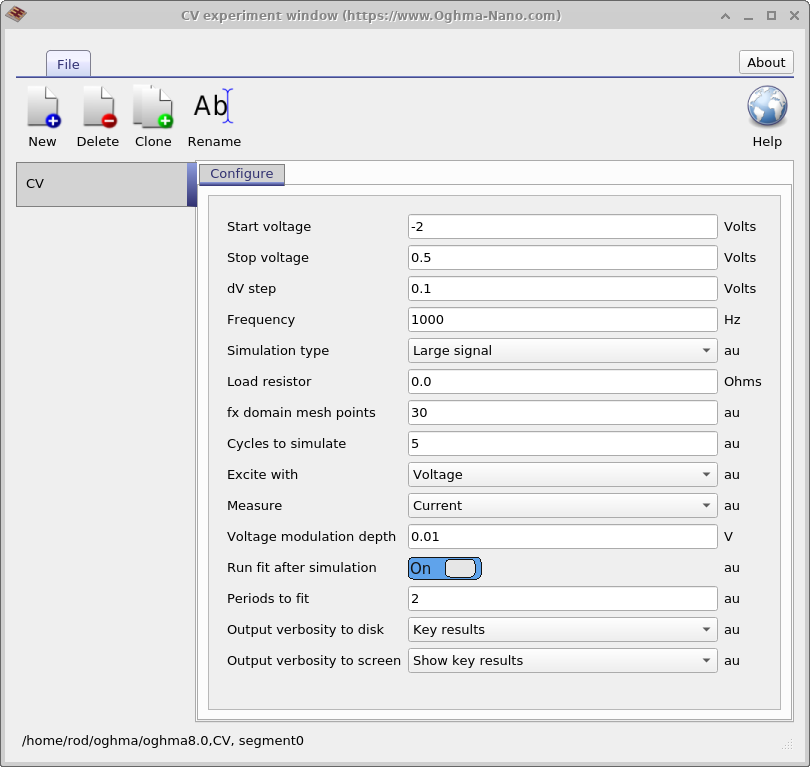
\includegraphics[width=0.7\textwidth,height=0.5\textwidth]{./images/sim_editors/cv.png}
\caption{The capacitance voltage editor}
\label{fig:cv_editor}
\end{figure}

\subsection{Outputs}

\begin{table}[H]
\begin{center}
\begin{tabular}{ |c|c| } 
 \hline
	File name 		& 	Description  \\ 
 \hline
	real\_imag.dat 		&	Re(i(fx)) v.s. Im(i(fx)) \\ 
	fx\_real.dat 		&	fx v.s. Re(i(fx)) \\ 
	fx\_imag.dat 		&	fx v.s. Im(i(fx)) \\ 
	cv.dat 				&	fx v.s. Capacitance \\ 
	cv2.dat 			&	fx v.s. $1/{Capacitance}^2$ \\ 
 \hline
\end{tabular}
\caption{Files produced by the CV simulation}
\label{tab:suns_jsc_output}
\end{center}
\end{table}


